% -----------------------------------------------------------------------------------------
\vspace{5mm}
{\color{lightgray} \hrule}
\begin{enumerate} \setcounter{enumi}{4}
	\item Implementar el algoritmo Adaptive Rejection Sampling y simular de una $Gamma(2,1)$ $10,000$ muestras. ¿cuando es conveniente dejar de adaptar la envolvente? [6 puntos]
\end{enumerate}

\textcolor{BrickRed}{\it Respuesta:}

Sabemos que ARS es un método de muestreo que utiliza una envolvente superior de la función objetivo para proponer muestras y luego decidir si aceptarlas o no mediante el criterio de aceptación/rechazo. Esto se implementa en el archivo  \textcolor{mediumblue}{ARS.py}.

Debido a la cantidad de código, se propone la creación de un diccionario que almacene los parámetros del método ARS y las funciones auxiliares. De esta forma, se puede acceder a los valores de los parámetros y las funciones de manera más sencilla. Además, se propone la creación de una función que inicialice los parámetros del método ARS y los guarde en el diccionario. Por último, se propone la creación de una función que genere muestras de la distribución log-concava usando el método ARS y actualice los parámetros del diccionario a medida que se generan muestras.

\textbf{Nota:} Primero se revisará, a grandes rasgos, un poco de lo visto en clase para entender mejor cada parte del código:

Sean
\begin{itemize}
	\item $f(x)$ la función proporcional a la densidad objetivo de la que se quiere muestrear.
	\item $h(x) = \log{(f(x))}$ el logaritmo de la función objetivo (es una función cóncava) con derivada $h'(x)$.
	\item $\mathcal{S}_n$ un conjunto de puntos $x_{i}$ con $i = 0,\dots n+1$ en el soporte de $f$ tales que $h(x_i) = \log{(f(x_i))}$ se conoce hasta una constante.
	\item $\mathcal{L}_{i}(x)$ la recta con pendiente $h^{'}(x_{i})$ que pasa por el punto $(x_i, h(x_i))$, es decir, la recta tangente a $h$.
\end{itemize}

Notemos que $\mathcal{L}_{i}$ siempre está por encima de $h$, esto es posible gracias a la concavidad de $h$.
\begin{figure}[h!]
	\centering
	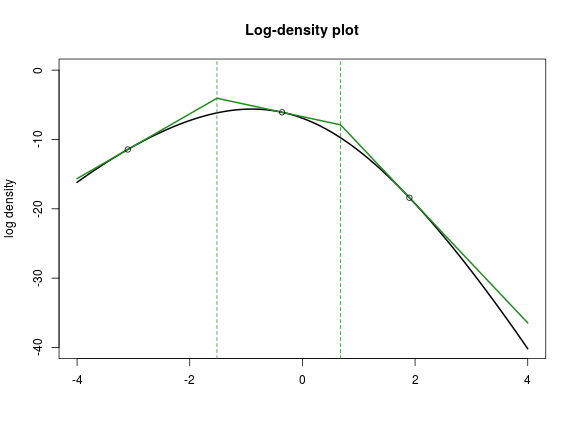
\includegraphics[width=0.65\textwidth]{IMAGENES/libro}
\end{figure}

\textbf{Intersecciones entre las $\mathcal{L}$'s}

Notemos que en cada intervalo $[x_i, x_{i+1}]$, se tiene un par de rectas tangentes correspondientes a $x_i$ y $x_{i+1}$. Además cuentan con una intersección para algún punto $z_i\in[x_i, x_{i+1}]$ (ver imágen anterior). Por la ecuación de la recta que úne dos puntos, tenemos que estas rectas están dadas por
\begin{equation}
	\mathcal{L}_{i} (x)= h(x_{i}) + h^{'}(x_{i}) (x - x_{i}) \text{ y } \mathcal{L}_{i+1} (x) =  h(x_{i+1}) + h^{'}(x_{i+1}) (x - x_{i+1})
\end{equation}
Entonces, la intersección es aquel $z_i$ tal que cumpla ambas ecuaciones anteriores. Después de igualar estas expresiones y hacer los cálculos necesarios, se tiene que:
\begin{equation}\label{eq:7}
	z_{i} = -\frac{h_{i+1} - h_{i} - \left(h_{i+1}^{'} x_{i+1} - h_{i}^{'} x_{i}\right)}{h_{i+1}^{'} - h_{i}^{'}}
\end{equation} 
donde $h_{j} = h(x_{j})$ y $h_{j}^{'} = h^{'}(x_{j})$. De esta forma, la envolvente superior está dada por:

$$	
	u(x) :=
	\begin{cases}
		h(x_0) + h^{'}(x_0)(x-x_0) = \mathcal{L}_{0} (x) & \text{si } x \leq z_0, \\
		\hspace{3cm}\vdots \\
		h(x_i) + h^{'}(x_i)(x-x_i) = \mathcal{L}_{i} (x) & \text{si } z_{i} \leq x \leq z_{i+1}, \\
		\hspace{3cm}\vdots \\
		h(x_n) + h^{'}(x_n)(x-x_n) = \mathcal{L}_{n} (x) & \text{si } z_n \leq x, \\
	\end{cases}
$$
y la envolvente en cada punto de intersección es
\begin{equation} \label{eq:8}
	u_{i} := \mathcal{L}_{i} (z_{i}).
\end{equation} 

\newpage
\textbf{Área bajo las rectas tangentes}

A continuación, se necesitan calcular los segmentos de área bajo las rectas tangentes de la envolvente superior, o bien, el área acumulada bajo las tangentes de la envolvente superior. Esto es necesario para normalizar las probabilidades durante el proceso de muestreo:

Se tiene que $u(x) = \mathcal{L}_{i} (x)$ en $[x_i, x_{i+1}]$, así
\begin{equation*}
	e^{u(x)} = e^{\mathcal{L}_{i} (x)} = e^{h(x_{i}) + h^{'}(x_{i}) (x - x_{i})} = e^{h(x_{i})} e^{h^{'}(x_{i}) (x - x_{i})}
\end{equation*}
El área bajo la curva $e^{u(x)}$ en $[x_i, x_{i+1}]$ es:
\begin{equation} \label{eq:9}
	e^{h(x_{i})} \int_{x_{i}}^{x_{i+1}}  e^{h^{'}(x_{i}) (x - x_{i})} dx = e^{h(x_{i})} \frac{e^{h^{'}(x_{i}) (x_{i+1} - x_{i})} - 1}{h^{'}(x_{i})} = \frac{e^{u(x_{i+1})} - e^{u(x_{i})}}{h^{'}(x_{i})},
\end{equation}
ya que $u(x_{i+1}) = h(x_{i}) + h^{'}(x_{i}) (x_{i+1} - x_{i})$. Entonces, la suma acumulada de estos términos es:
\begin{equation}\label{eq:10}
	s_{j} := \sum_{i=1}^{j}  \frac{e^{u(x_{i+1})} - e^{u(x_{i})}}{h^{'}(x_{i})}.
\end{equation}
Y la última suma acumulativa es: 
\begin{equation} \label{eq:11}
	cu_i := s_{n}.
\end{equation}

\vspace{5mm}
\begin{center}
	\textcolor{mediumblue}{----------- ARS.py -----------}
\end{center}

A continuación, se da una descipción detallada de lo que hacen las funciones implementadas en el archivo:

\begin{itemize}
\item Las expresiones \eqref{eq:7}, \eqref{eq:8}, \eqref{eq:10}, \eqref{eq:11} se calculan con la función auxiliar \textit{intersecciones\_y\_areas()}, la cual nos ayuda a hacer estos cálculos para una muestra dada de $x_i$, sus evaluaciones $h(x_i)$ y sus pendientes $h^{'}(x_i)$. 

\item Posteriormente, se da la función \textit{DIC\_INICIAL()} la cual crea un diccionario con los parámetros iniciales para el método de muestreo de Adaptive Rejection Sampling (ARS).
Inicializa los puntos $x_i$, los valores $h(x_i)$, sus pendientes $h^{'}(x_i)$ y usa la función \textit{intersecciones\_y\_areas()} para calcular los puntos de intersección $z_i$ de las tangentes. Además, calcula la envolvente superior $u(x) = h(x_i) + h^{'}(x_i) (x - x_i)$ y el área acumulada $s_i$ bajo las tangentes. El área acumulada hasta el último punto se guarda en $cu_i$. Esta función regresa el diccionario de parámetros inicializados.

\item Después, se tiene la función \textit{muestreo()} la cual devuelve un solo valor muestreado aleatoriamente desde la envolvente superior de la función log-concava que está siendo muestreada y el índice del segmento en el que cayó el valor muestreado. Genera un número aleatorio $u\sim\mathcal{U}(0,1)$ y este se utiliza para seleccionar un punto en la envolvente superior, basándose en las áreas acumuladas bajo las rectas tangentes que representan la envolvente superior ya que se quiere encontrar en qué segmento de la envolvente superior se encuentra el valor de $u$:
\begin{equation} \label{eq:12}
	i = \max \left\{ j \mid \frac{s_j}{cu_{i}} < u \right\}
\end{equation}
La función usa el concepto de muestreo inverso por transformada. Al generar un número aleatorio  $u$, se busca un punto cuya área acumulada (normalizada) hasta dicho punto sea igual a $u$ (como el ejemplo contructivo visto en clase). Una vez identificado el segmento adecuado, se muestrea un punto dentro de ese segmento usando las propiedades locales de la función log-convexa (como las pendientes y las alturas).

Una vez encontrado el segmento $i$, se calcula el punto  $x_t$  dentro de ese segmento de la envolvente superior. Para esto, se usa la fórmula:
\begin{equation} \label{eq:13}
	x_t = x_i + \frac{-h(x_i) + \log \left( h^{'}(x_i) \cdot \left( cu_i \cdot u - s_i \right) + e^{u_i} \right)}{h^{'}(x_i)}
\end{equation}
Esta se obtuvo gracias a que, ya habíamos visto que para $x_t\in[x_{i}, x_{i+1}]$, entonces
\begin{equation*}
	\int_{x_{i}}^{x_t} e^{u(x)} dx =  \frac{e^{u(x_t)} - e^{u(x_{i})}}{h^{'}(x_{i})}
\end{equation*}
y se quiere que esta área acumulada se corresponda con el número aleatorio $u$ generado en $[0, 1]$, es decir, se necesita resolver la ecuación:
\begin{equation*}
	\frac{e^{u(x_t)} - e^{u(x_{i})}}{h^{'}(x_{i})} = cu_i \cdot u - s_i.
\end{equation*}
Resolviendo esta ecuación para $x_t$, de obtiene le expresión \eqref{eq:13}.

\item En la función \textit{insertar\_puntos()} se actualizan las envolventes con nuevos puntos. Si no se proporcionan, solo recalcula la envolvente a partir de los puntos existentes. Si se proporcionan nuevos puntos, se concatenan con los existentes y se recalcula la envolvente. Además, se recalculan los puntos de intersección de las tangentes y el área acumulada bajo la
envolvente con ayuda de la función auxiliar \textit{intersecciones\_y\_areas()}.

\item Finalmente, se tiene la función \textit{aceptacion\_rechazo()}. La cual genera $N$  muestras a partir de la envolvente superior y actualizarla si es necesario. Esta función implementa el muestreo adaptativo, aprovechando el método ARS. La lógica se basa en aceptar o rechazar muestras propuestas de acuerdo con la envolvente superior y la función subyacente. Usa a la función \textit{muestreo()} para obtener una propuesta de muestra  $x_t$  y el índice del segmento de la envolvente superior donde está situada. Calcular la altura de la envolvente superior en  $x_t$, luego, genera un número aleatorio $u\sim\mathcal{U}$ para decidir si se acepta $x_t$ o no. Esto se logra comparando a $u$ con la probabilidad de aceptación:
\begin{equation} \label{eq:14}
	\exp{\left(h(x_t)-u(x_t)\right)}
\end{equation}
(Esto se deriva de la relación entre la envolvente superior y la función objetivo). Si
\begin{equation} \label{eq:15}
	u <	\exp{\left(h(x_t)-u(x_t)\right)}
\end{equation}
se acepta la muestra y se almacena y se actualiza $\mathcal{S}_n$.
\end{itemize}

\textbf{Ejemplos de uso:}
	
Al final del archivo \textcolor{mediumblue}{ARS.py} se tiene un par de ejemplos:
\begin{itemize}
	\item Generación de una distribución normal $X\sim\mathcal{N}(2,3)$. Para esto, necesitamos $h$ cóncava tal que $e^{h}$ sea proporcional a la distribución de $X$. Para esto, se propone una alteración de la distribución Log Normal:
	\begin{equation}
		h(x,\mu,\sigma) = -\frac{(x-\mu)^2}{2\sigma^{2}}
	\end{equation}
	con derivada:
	\begin{equation}
		h^{'}(x, \mu, \sigma) = -\frac{(x-\mu)}{\sigma^2}
	\end{equation}
	Notemos que $e^{h(x)} \propto \mathcal{N}(\mu,\sigma)$. Se obtuvo el siguiente resultado y se comparó con la distribución verdadera $X\sim\mathcal{N}(2,3)$:
	
	\begin{figure}[h!]
		\centering
		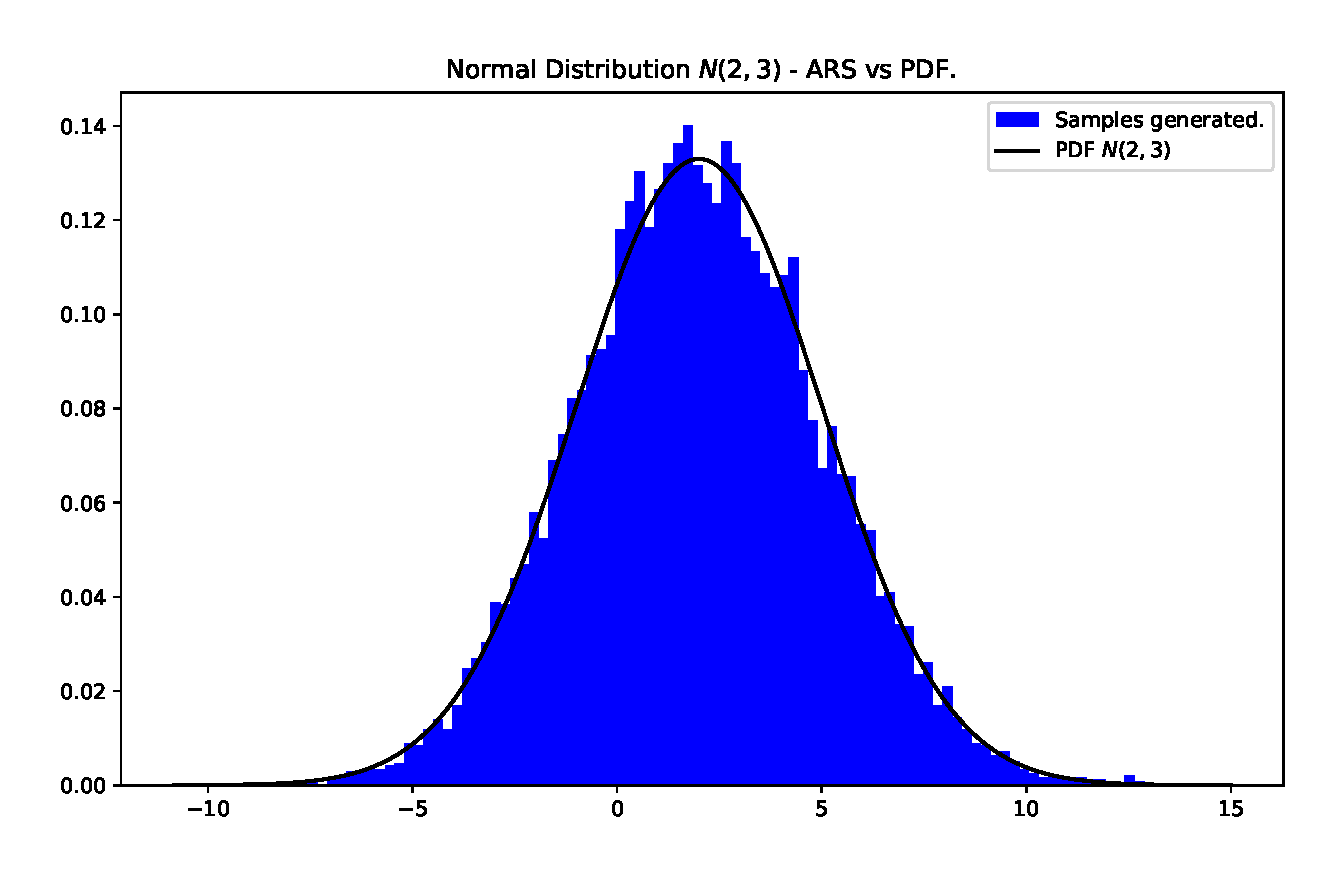
\includegraphics[width=0.59\textwidth]{IMAGENES/ARS_example1.pdf}
	\end{figure}
	
	\item De la misma forma, se generó una distribución $Beta(1.3,2.7)$:
	\begin{figure}[h!]
		\centering
		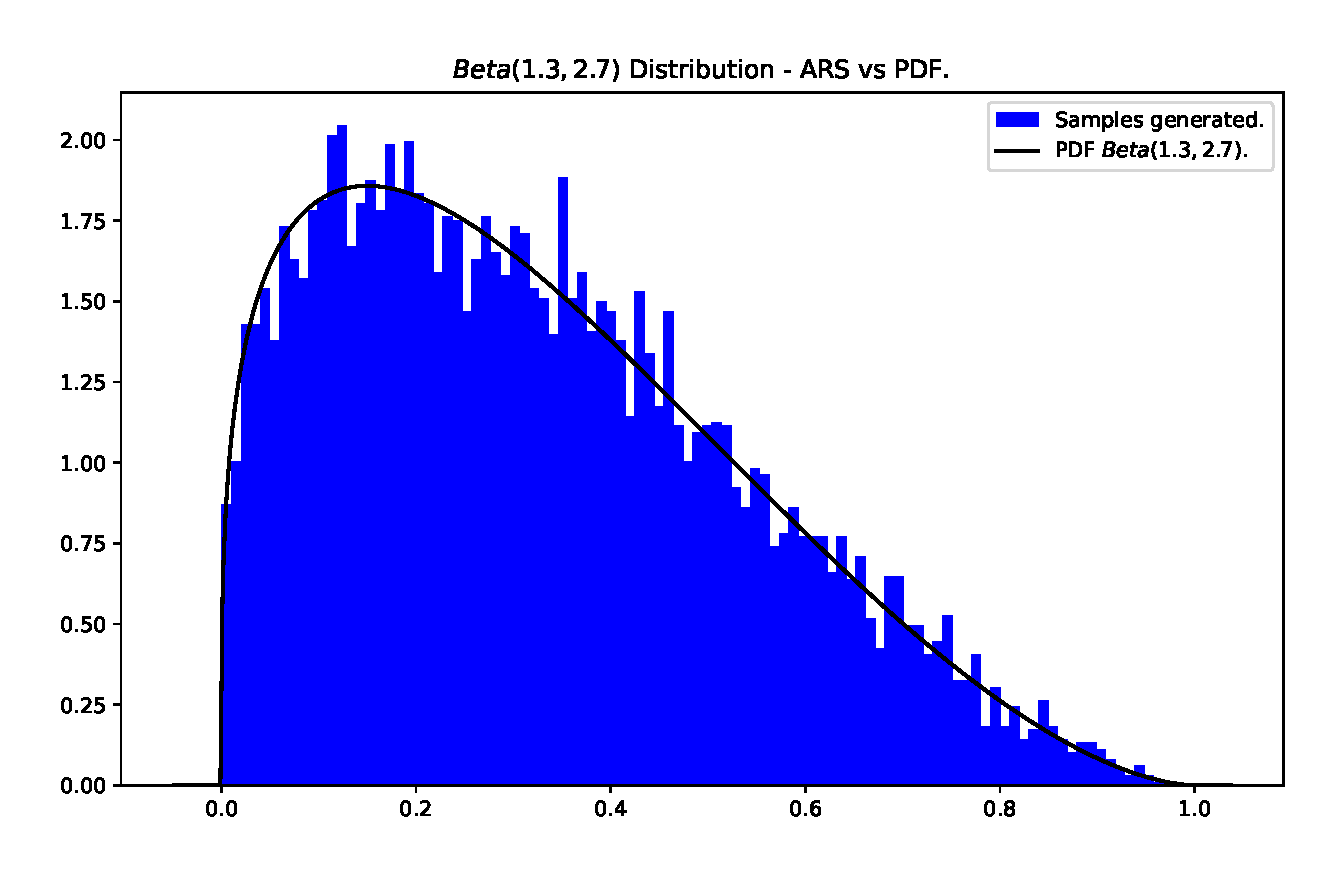
\includegraphics[width=0.59\textwidth]{IMAGENES/ARS_example2.pdf}
	\end{figure}
\end{itemize}

\textbf{Distribución $Gamma(2,1)$}

Para generar esta distribución, en el archivo \textcolor{mediumblue}{ejercicio5\_tarea5.py}, se propone el uso de
\begin{equation}
	h(x,k, \theta) = (k-1)\log{x} - \frac{x}{\theta}
\end{equation}
con derivada:
\begin{equation}
	h^{'}(x,k,\theta) = \frac{k-1}{x} - \frac{1}{\theta}
\end{equation}
En la cual podemos notar que
\begin{equation}
		e^{h(x)} = e^{(k-1)\log{x} - \frac{x}{\theta}} = x^{k-1} e^{-\frac{x}{\theta}} \propto \frac{1}{\Gamma(k) \theta^{k}} x^{k-1} e^{-\frac{x}{\theta}}
\end{equation}
que es la distribución de $X\sim Gamma(k,\theta)$. Esto se usa en \textcolor{mediumblue}{ejercicio5\_tarea5.py} para generar $N=10000$ muestras de $Gamma(2,1)$, para los puntos iniciales: $\mathcal{S} = \{0.1,0.5,2,5,10\}$ en el soporte de $X$. Esto nos genera:

\begin{figure}[h!]
	\centering
	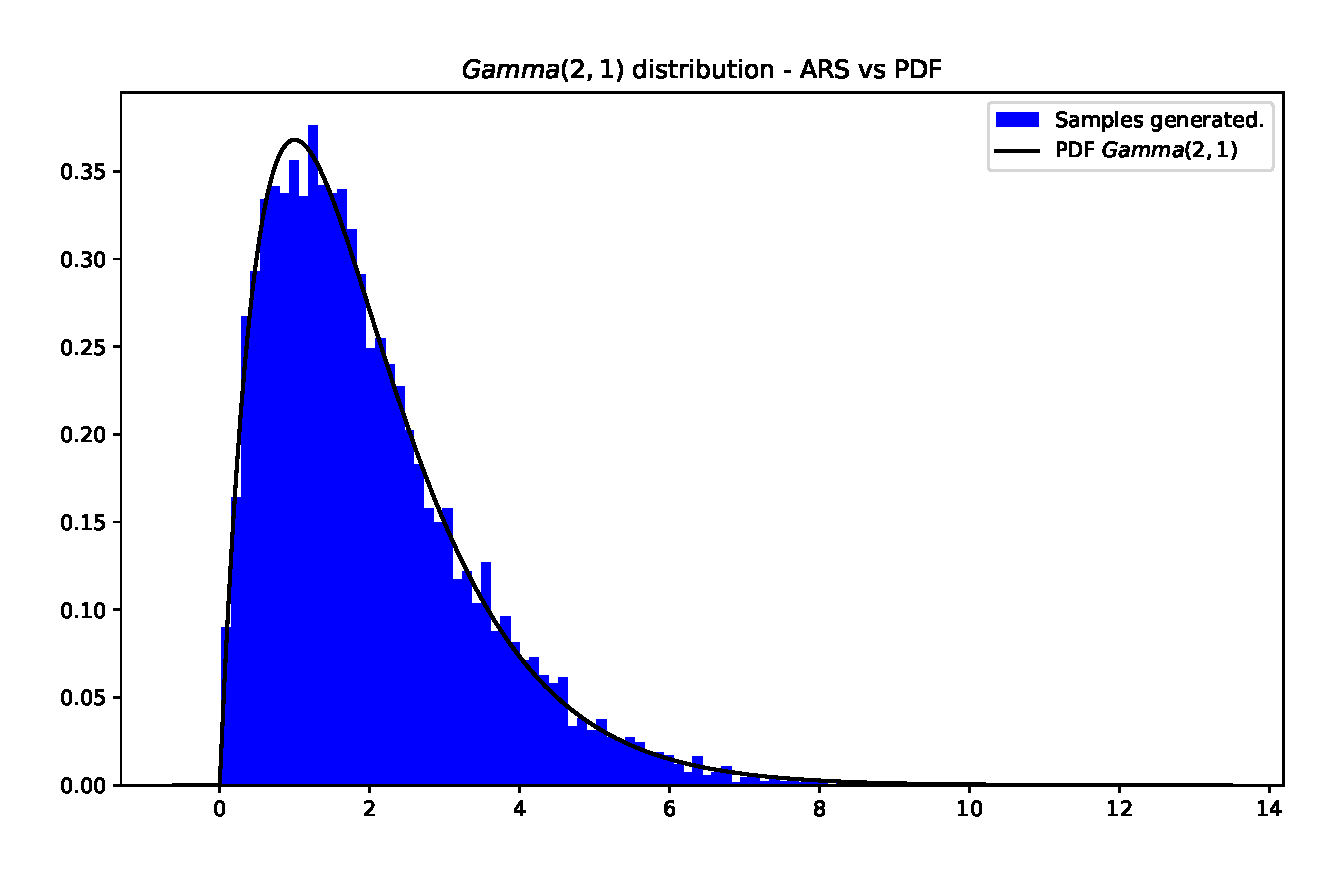
\includegraphics[width=0.59\textwidth]{IMAGENES/ARS_gamma.pdf}
\end{figure}

Para responder la pregunta ¿cuándo es conveniente dejar de adaptar la envolvente?:

En ARS, inicialmente se utilizan algunos puntos para definir la envolvente superior (compuesta por segmentos lineales), pero después, cada vez que se rechaza un valor propuesto o cuando se detecta que la envolvente puede mejorar, se añaden nuevos puntos de tangencia.

Si el criterio de rechazo se cumple en una proporción suficientemente baja (es decir, la mayoría de las muestras propuestas son aceptadas), significa que la envolvente ya está ajustada de manera adecuada. En este caso, puedes dejar de adaptar la envolvente porque el proceso de muestreo es eficiente. O bien, fijar un límite máximo para el número de puntos para mejorar el costo computacional. En mi implementación se usó un número máximo de $100$ puntos.